\chapter{Estado de la Cuestión}
\label{cap:estadoDeLaCuestion}
En este capítulo se presenta el estado del arte de los distintos elementos que componen el trabajo. Estos campos son la comunicación no verbal en entornos virtuales, la captura de movimiento, distintos modelos de \gls{ia}, motores de videojuegos y el estado actual de los entornos virtuales.

\section{Entornos virtuales}
Como se puede ver en el artículo \cite{NOVE}, se empezó a hablar en la década de los 90 de entornos virtuales y el \gls{metaverso} como nuevas formas de comunicarse con las personas.
Estos entornos virtuales al principio eran muy sencillos, con pocas actividades que realizar y el chat escrito como única forma de comunicarse. Algún ejemplo de estos entornos virtuales eran el Second Life o el Habbo Hotel.

Para continuar hablando de los entornos virtuales es necesario introducir los conceptos de ``inmersión'' y ``presencia'': dos términos que, a menudo se usan como sinónimos, pero son ligeramente distintos aunque están muy relacionados.
Como lo define el artículo \cite{MRPI}, la presencia es la calidad experimental en entornos virtuales; mientras que la inmersión está asociado con los aspectos técnicos de un sistema virtual que ayudan al usuario a potenciar la sensación de presencia.
Estudios recientes como \cite{FPPS} demuestran como la presencia, tanto la nuestra propia como la social, son potenciadores del apoyo social percibido, lo que se asocia con el bienestar de los usuarios; mientras que el estudio \cite{GVR} muestra que, aunque no haya mejoras performáticas entre jugar en entornos inmersivos (\gls{vr}) y no inmersivos (un ordenador), los jugadores encontraron más emocionantes y con mayor presencia los entornos interactivos.
Es por esto último que con la aparición de la \gls{vr} se hicieron populares entornos virtuales focalizados en esta tecnología.

Con todo esto es natural que las empresas inviertan en tecnologías que aumenten la sensación de inmersión para lograr una mayor presencia.
Empresas como Apple o Meta están apostando en la tecnología \gls{vr}, sacando recientemente las gafas Apple Vision Pro (2024) y Meta Quest 3 (2023); mejorando aspectos como la calidad de las cámaras, el sonido, el reconocimiento de gestos y su comodidad que pueden amplificar la sensación de inmersión cuando se utilizan.
Además, Meta está centrada en la idea de \gls{metaverso} como un espacio digital en el que se puede socializar.

Con la idea de mejorar la inmersión en entornos virtuales se ideó este proyecto en el que, mediante la captura de movimiento, se puede usar la comunicación no verbal para expresar ciertas acciones y el entorno sea capaz de reconocer lo que estamos haciendo. Todo esto pensado para que se pueda usar en entornos de \gls{vr} para llevar la inmersión al máximo

%Dejo esto por aquí a ver qué te parecen estos apartados para hablar de ellos
\section{Comunicación no verbal en entornos virtuales}
En los últimos años se han llevado a cabo distintos estudios sobre la comunicación no verbal en entornos virtuales. El estudio \cite{XGKD23} se centra en el concepto de presencia en entornos virtuales, enfatizando los roles de inmersión, contenido emocional y fidelidad de avatares en la mejora de la experiencia del usuario. El estudio resalta como el realismo de los avatares y sus comportamientos (movimiento y lenguaje corporal) ayudan a conseguir un mayor sentimiento de presencia social entre los usuarios. También se discute como estos elementos influyen en las dinámicas interpersonales  y la percepción del usuario en entornos virtuales.

Estos roles discutidos en el estudio pueden extrapolarse a la experiencia de jugar a videojuegos. En el contexto de los videojuegos tradicionales, las opciones de comunicación no verbal son las dadas por los desarrolladores en forma de gestos, acciones dentro del juego (agacharse, girar su avatar o mover la cabeza al mover la cámara por ejemplo). Dentro de cada videojuego la comunidad va a intentar usar las opciones que se les proporcione para comunicarse entre ellos mismos de la mejor manera posible.

Un ejemplo claro de evolución de la comunicación no verbal en videojuegos y su importancia para los jugadores es el caso de \textit{VR chat}. \textit{VR chat} es un videojuego \gls{mmorpg} de \gls{vr} donde los jugadores pueden unirse a distintos mundos e interactuar con otros usuarios. Este juego no solo permite el uso de gafas de \gls{vr}, sino que también permite (de manera experimental) usar distintas formas de captura de movimiento de cuerpo completo \footnote{Enlace a la documentación de \textit{VR Chat} para su \gls{sdk} de captura de movimiento de cuerpo completo \cite{VRCHATSDK}}.

Los usuarios de esta aplicación han buscado distintas formas de conseguir una mayor expresividad en sus avatares para así poder entablar mejor conversaciones entre ellos o para poder expresarse como les gustaría. Algunos de estos métodos se describen en el siguiente apartado junto a métodos de captura de movimiento no orientados a videojuegos.

\section{Captura de movimiento}

La captura de movimiento es una técnica que permite digitalizar el movimiento de una persona. Esta técnica se usa sobre todo en el ámbito de la animación, el cine y los videojuegos.
Para lograr esto se han desarrollado diferentes tipos de tecnologías: óptica, mecánica y magnética.

\subsection{Captura de movimiento óptica}
La captura de movimiento óptica consiste en el uso de cámaras para la captura.
Según el artículo \cite{OPTICAL} esta captura se puede dividir en monocular o multivista dependiendo del número de cámaras, y según si utilizan marcadores o no.
En el mismo artículo explica el funcionamiento de la captura óptica multivista con el uso de marcdores, el cual se utiliza en gran medida en la industria audiovisual.
Este tipo de captura óptica necesita al menos de un conjunto de cámaras sincronizadas (dos o más), un traje con marcadores en puntos significativos (articulaciones sobretodo) y un sistema de adquisición de varios vídeos simultáneos.
La reconstrucción del movimiento se basa en la sincronía de las cámaras y la capacidad de detección de los mismos marcadores desde diferentes puntos de vista, haciendo que se pueda reconstruir en 3D los marcadores mediante la triangulación de los distintos puntos de vista.

Un ejemplo de la captura de movimiento óptica monocular y sin marcadores son los sistemas basados en cámaras 3D que utilizan los \gls{IRs} para calcular la profundidad. Según el artículo \cite{KINECT} la Kinect (Microsoft, 2010) utilizaba esta tecnología para ello.
Consiste en un proyector de \gls{IRs} cuyos rayos atraviesan una rejilla de difracción, convirtiéndose en un conjunto de puntos que, como se sabe la geometría relativa entre este proyector y una cámara de \gls{IRs} que venía incorporada, se podía triangular la posición de un objeto haciendo coincidir un punto observado con uno de los puntos del proyector.

\subsection{Captura de movimiento mecánica}
La captura de movimiento mecánica se consigue mediante sensores inerciales.
Según se puede ver en \cite{XSENS}, el traje Xsens MVN es un ejemplo de ello.
No utiliza cámaras o marcadores si no la combinación de giroscopios, acelerómetros y magnetómetros.
Con los datos recibidos de estos sensores se puede estimar la rotación de los diferentes puntos, mientras que la posición se puede estimar mediante supuestos de una cadena cinemática.
En la figura \ref{fig:XSensTraje} se puede ver el traje visto desde la espalda.

\begin{figure}[H]
    \centering
    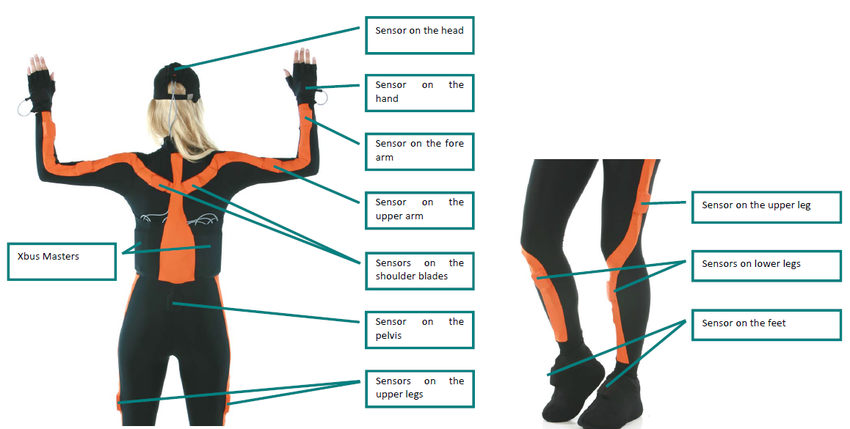
\includegraphics[width=0.5\textwidth]{Imagenes/Bitmap/XSens.png}
    \caption[Imágen del traje de captura de movimiento XSens]{Imágen del traje de captura de movimiento XSens \footnotemark }
    \label{fig:XSensTraje}
\end{figure}

\footnotetext{Fuente de la imagen: \url{https://www.researchgate.net/figure/The-Xsens-MVN-full-body-motion-capture-suit-Picture-source-htttp-wwwxsenscom_fig1_233926874}}

\subsection{Captura de movimiento magnética}
La captura magnética se consiste mediante sensores electromagnéticos.
El artículo \cite{EMS} explica que la generación de valores en un campo electromagnético tridimensional es suficiente para determinar la posición y rotación de un objeto emisor frente a un sensor.
Para ello se aplican transformaciones lineales a la excitación de la fuente y los vectores recibidos por el receptor para percibir pequeños cambios en los valores a determinar, los cuales se separan mediante combinaciones lineales de los vectores de salida del sensor y se utilizan para actualizar las coordenadas previas.

En esta última tecnología se basa el traje Perception Neuron 3.
Este traje fue creado por Noitom, empresa fundada en el 2012 enfocada en el desarrollo de tecnología de captación de movimiento.
El traje previamente mencionado se encuentra dentro de la serie de trajes ``Perception Neuron'', los cuales son bandas de velcro a las que se pueden acoplar sensores electromagnéticos.

\section{Motores de videojuegos}
Un motor de videojuegos es un software que proporciona herramientas para desarrollar y ejecutar un videojuego.
Estos motores están compuestos a su vez de otros motores más específicos que se encargan de funcionalidades básicas para un videojuego para que el desarrollador del juego no tenga que encargarse de ello. Algunos ejemplos de esto último son el motor de render, el de físicas o el de sonido.

Actualmente los motores de videojuegos más usados en el mercado son Unity, Unreal y Godot.
Aunque el artículo \cite{SGE} no se centre en un análisis del mercado en general, si contiene varias estadísticas sobre el uso de los principales motores de videojuegos en el mercado en 2023.
Este artículo menciona que, de los juegos publicados en Steam ese año, un 60.04\% fueron hechos en Unity, un 16.42\% fueron hechos en Unreal y el 23.54\% restante fue hecho en motores propios de empresas (Source o CryEngine, por ejemplo).

\subsection{Unity}
Unity es un motor de videojuegos creado por Unity Technologies en 2005. A continuación se listan las principales herramientas que usa el motor:

\begin{enumerate}
    \item Motor gráfico: Propio de Unity basado mayoritariamente en OpenGL (para depende de qué plataformas puede usar otro, como Direct3D para Windows).
    \item Motor físico: PhysX, creado por la empresa Nvidia Corporation.
    \item Motor de audio: Propio de Unity.
    \item Lenguaje de scripting: C\#.
    \item Lenguaje de scripting de shaders: ShaderLab.
\end{enumerate}

El modelo clásico de Unity se ha basado en la arquitectura Entidad-Componente (EC).
Esta arquitectura deja a todo lo que hay en el juego (las entidades, llamadas en Unity ``GameObjects'') como contenedores de componentes, que son los que le aportan funcionalidad a éstas.
Este modelo supuso una mejoría ante la programación de videojuegos con objetos, ya que conseguía independizar comportamientos.

Desde 2022 mediante el paquete Unity DOTS (Data-Oriented Technology Stack) \footnote{Enlace a la documentación del paquete DOTS: \url{https://docs.unity3d.com/Packages/com.unity.entities@1.3/manual/index.html}} se pueden crear videojuegos siguiendo la arquitectura Entidad-Componente-Sistema (ECS).
Esta arquitectura consiste en separar la lógica de los datos, ya que los datos se guardan en componentes mientras que la lógica la ejecutan los sistemas.
ECS supone una mejoría a EC gracias a la separación mencionada, ya que mejora la escabilidad del código y la modularidad.

\subsection{Unreal}
Unreal es un motor de videojuegos creado por Epic Games en 1998 con el lanzamiento de Unreal Engine 1.
La versión estable actual es Unreal Engine 5.5, lanzada en noviembre de 2024.
El código fuente de este motor está escrito en C++ y es accesible desde Github \footnote{Enlace a la página de Github de Epic: \url{https://github.com/epicgames}}.
Las principales herramientas del motor son:


\begin{enumerate}
    \item Motor gráfico: Propio de Unreal. Este cuenta con  tecnologías para optimizar geometría (Nanite), sistema de iluminación dinámica (Lumen), y una técnica de escalado de imágenes (TSR)
    \item Motor físico: Chaos Physics, desarrollado por Epic Games para mejorar la integración con las diferentes herramientas del motor.
    \item Motor de audio: Propio de Epic Games llamado MetaSounds.
    \item Lenguaje de scripting: C++ y Blueprints como scripting visual.
    \item Lenguaje de scripting de shaders: High-Level Shading Language (HLSL) y Material Editor como forma de abstracción, permitiendo crear materiales con nodos visuales.
\end{enumerate}

Unreal utiliza una arquitectura orientada a clases jerárquicas más cercana a la programación orientada a objetos con alguna integración con componentes.
Los objetos del mundo, llamados ``actores'', heredan de la clase AActor y son los componentes quienes le dan alguna de las funcionalidades (mallas, físicas o cámara por ejemplo).
Las clases controlables (tanto por el jugador como por \gls{ia}) son entidades de tipo ``Pawn'' (clase APawn), de la cual hereda los objetos de tipo ``Character'' (clase ACharacter), los cuales tienen un movimiento humanoide incorporado.
Para introducir movimiento a los objetos Pawn es necesario hacerlo mediante objetos de tipo controller (APlayerControler para entrada de input y AAIController para \gls{ia}).

\section{Modelos de \gls{ia}}

La inteligencia artifical ha sido un tópico de desarrollo e investigación en los útlimos años. Aunque el desarrollo en los últimos años se ha centrado sobre todo en el ámbito de las \glspl{ia} generativas, este estudio se va a centrar sobre todo en el uso de redes neuronales e \glspl{ia} de clasificación más tradicionales.

\subsection{Tecnologías de \gls{ia}}

En la actualidad, el mundo de la \gls{ia} está centrado en el desarrollo en python mediante el uso de librerías programadas en C++. Las librerías más comunes son Tensorflow, Pytorch y scikit-learn.

Tensorflow tiene un enfoque más orientado a la producción y despliegue de modelos de \gls{ia} a un nivel empresarial, pytorch es más usado en el ámbito académico y de investigación por su capacidad de rápido prototipado. Scikit-learn se usa más para enseñar los principios de la \gls{ia} y desarrollar modelos más ligeros y más tradicionales.

Estas librerías se usan en conjunto con Numpy(\cite{harris2020array}) y Pandas(\cite{reback2020pandas}, \cite{mckinney-proc-scipy-2010}) para conseguir unos cálculos más efectivos sobre la gran cantidad de datos que se necesitan en el ciclo de vida de un modelo de \gls{ia}.

\subsection{Librerías de \gls{ia}}

En el apartado anterior ya se han nombrado distintas librerías de \gls{ia} que se usan en la actualidad. En este apartado se van a describir las más relevantes para el desarrollo de este trabajo.

\subsubsection{Tensorflow}

Tensorflow(\cite{tensorflow2015-whitepaper}) es una libería de \gls{ia} desarrollada y mantenida por el equipo de Google Brain desde 2015. Esta librería permite el desarrollo de modelos de \gls{ia} usando \glspl{cpu}, \glspl{gpu} y \glspl{tpu}. Tensorflow es una plataforma de código abierto que tiene un ecosistema de herramientas y librerías que permite el desarrollo e investigación de modelos de \gls{ia}.
Tensorflow tiene un enfoque más orientado a la producción y despliegue de modelos de \gls{ia} a un nivel empresarial, por lo que es más común ver su uso en empresas que en el ámbito académico. Un ejemplo de este enfoque es la presencia de la herramienta Tensorflow Serving \cite{olston2017tensorflowservingflexiblehighperformanceml}, que permite el desplegado de modelos de Tensorflow (o compatibles con el ecosistema) de una forma sencilla.

\subsubsection{PyTorch}
PyTorch(\cite{Ansel_PyTorch_2_Faster_2024}) fue desarrolladapor Facebook AI Research en 2026, se hizo de código abierto en 2017 y en 2022 se unió a la Linux Fundation. Esta librería se centra en la idea de que la búsqueda de usabilidad y velocidad son compatibles. Pytorch permite el desarrollo de modelos de \gls{ia} al igual que Tensorflow, pero su modelo de código y desarrollo ha hecho que se use más para prototipado rápido y desarrollo de proyectos dinámicos.
Pytorch permite la integración con otras librerías como NumPy, SciPy y Cython, lo que permite un desarrollo más rápido y sencillo de modelos de \gls{ia}.

\subsubsection{Scikit-learn}
Scikit-learn(\cite{scikit-learn}) es una librería de \gls{ia} desarrollada en Python que se centra en el aprendizaje automático. Esta librería se basa en NumPy, SciPy y matplotlib, lo que permite un desarrollo más sencillo de modelos de \gls{ia}. Scikit-learn es una librería más ligera y más tradicional que Tensorflow o Pytorch, por lo que es más común ver su uso en el ámbito académico y de investigación. Scikit-learn se centra más en el análisis de datos predictivo y también es de código abierto como las anteriores.

\subsubsection{YDF}
YDF (\cite{GBBSP23}) es una librería para entrenar, evaluar, interpretar y desplegar \gls{randomforest}, \glspl{gradientboosteddecisiontree}, \gls{cart} y \gls{isolationforest}. Esta librería esta intregrada con Tensorflow y keras, centra su desarrollo en la optimización de árboles de decisión y en hacer una \gls{api} concisa y moderna.

\subsection{Modelos de reconocimiento de gestos y poses}

Muchos modelos de \gls{ia} se han desarrollado para la detección de gestos y poses. Estos modelos pueden usar imágenes, videos, datos de sensores o esqueletos formados por puntos de referencia. En este apartado se van a destacar los más relevantes para el resto del trabajo.

\subsubsection{YoLoV11}
YoLoV11(\cite{Jocher_Ultralytics_YOLO_2023}) es un conjunto de modelos \gls{yolo}, entre los que se encuentra un modelo de detección de poses. Por defecto este modelo usa 17 puntos de referencia (presentados en la tabla \ref{tab:pose-yolo}) y usa imágenes de 640x640 píxeles como entrada. En la página del modelo de pose\footnote{Página de YOLOv11-pose: \url{https://docs.ultralytics.com/es/tasks/pose/}}, Ultralytics incluye los distintos modelos de pose y su rendimiento y requerimientos. Este modelo se ofrece preentrenado en distintos tamaños con la opción de re entrenarse usando un dataset con el formato especificado por Ultralytics\footnote{Página de especificación del formato del dataset: \url{https://docs.ultralytics.com/es/datasets/pose/}}

\newpage

\begin{table}[H]
    \centering
    \caption{Puntos de referencia del modelo YOLOv11-pose}
    \label{tab:pose-yolo}
    \rowcolors{1}{white}{gray9}
    \begin{tabular}{|l|}
        \hline
        Nariz             \\
        \hline
        % \rowcolor{gray9}
        Ojo izquierdo     \\
        \hline
        Ojo derecho       \\
        \hline
        % \rowcolor{gray9}
        Oreja izquierda   \\
        \hline
        Oreja derecha     \\
        \hline
        % \rowcolor{gray9}
        Hombro izquierdo  \\
        \hline
        Hombro derecho    \\
        \hline
        % \rowcolor{gray9}
        Codo izquierdo    \\
        \hline
        Codo derecho      \\
        \hline
        % \rowcolor{gray9}
        Muñeca izquierda  \\
        \hline
        Muñeca derecha    \\
        \hline
        % \rowcolor{gray9}
        Cadera izquierda  \\
        \hline
        Cadera derecha    \\
        \hline
        % \rowcolor{gray9}
        Rodilla izquierda \\
        \hline
        Rodilla derecha   \\
        \hline
        % \rowcolor{gray9}
        Tobillo izquierdo \\
        \hline
        Tobillo derecho   \\
        \hline
    \end{tabular}
\end{table}

\subsubsection{Modelos para la detección del balance de personas andando}

En el artículo \cite{combining3dskeleton} se presenta una comparativa de modelos para la detección del balance de personas andando en distintos niveles de valance y con distintas restricciones con un traje usado. Este artículo presenta una generación de esqueletos en 3D a partir de una kinect y realiza una comparativa de distintos modelos tradicionales y neuronales para ver su efectividad. En las conclusiones podemos ver como, de los distintos modelos utilizados, el que mejor resultados da es un \gls{dcnn} que los investigadores proponen. Otros modelos de la comparativa incluyen el \gls{randomforest}, el \gls{svm}, \gls{lstm} y Naive Bayes en términos de modelos tradicionales. Otra comparativa se realiza con otros modelos basados en \glspl{cnn} como AlexNet, VGGNet y ResNet-18.

\subsubsection{Otros modelos de detección de gestos y poses}

En los últimos años se han desarrollado modelos generales de detección de gestos y poses. Estos modelos han tenido distintos enfoques, desde el uso de gafas de \gls{vr} para hacer detección de gestos simples con las manos para utilizarlos como método de entrada (Meta Quest 2 y 3 por ejemplo), a modelos de seguimiento de manos y distintos modelos de reconocimiento de Google con Gemini.